% Options for packages loaded elsewhere
% Options for packages loaded elsewhere
\PassOptionsToPackage{unicode}{hyperref}
\PassOptionsToPackage{hyphens}{url}
\PassOptionsToPackage{dvipsnames,svgnames,x11names}{xcolor}
%
\documentclass[
  letterpaper,
  DIV=11,
  numbers=noendperiod]{scrartcl}
\usepackage{xcolor}
\usepackage{amsmath,amssymb}
\setcounter{secnumdepth}{-\maxdimen} % remove section numbering
\usepackage{iftex}
\ifPDFTeX
  \usepackage[T1]{fontenc}
  \usepackage[utf8]{inputenc}
  \usepackage{textcomp} % provide euro and other symbols
\else % if luatex or xetex
  \usepackage{unicode-math} % this also loads fontspec
  \defaultfontfeatures{Scale=MatchLowercase}
  \defaultfontfeatures[\rmfamily]{Ligatures=TeX,Scale=1}
\fi
\usepackage{lmodern}
\ifPDFTeX\else
  % xetex/luatex font selection
\fi
% Use upquote if available, for straight quotes in verbatim environments
\IfFileExists{upquote.sty}{\usepackage{upquote}}{}
\IfFileExists{microtype.sty}{% use microtype if available
  \usepackage[]{microtype}
  \UseMicrotypeSet[protrusion]{basicmath} % disable protrusion for tt fonts
}{}
\makeatletter
\@ifundefined{KOMAClassName}{% if non-KOMA class
  \IfFileExists{parskip.sty}{%
    \usepackage{parskip}
  }{% else
    \setlength{\parindent}{0pt}
    \setlength{\parskip}{6pt plus 2pt minus 1pt}}
}{% if KOMA class
  \KOMAoptions{parskip=half}}
\makeatother
% Make \paragraph and \subparagraph free-standing
\makeatletter
\ifx\paragraph\undefined\else
  \let\oldparagraph\paragraph
  \renewcommand{\paragraph}{
    \@ifstar
      \xxxParagraphStar
      \xxxParagraphNoStar
  }
  \newcommand{\xxxParagraphStar}[1]{\oldparagraph*{#1}\mbox{}}
  \newcommand{\xxxParagraphNoStar}[1]{\oldparagraph{#1}\mbox{}}
\fi
\ifx\subparagraph\undefined\else
  \let\oldsubparagraph\subparagraph
  \renewcommand{\subparagraph}{
    \@ifstar
      \xxxSubParagraphStar
      \xxxSubParagraphNoStar
  }
  \newcommand{\xxxSubParagraphStar}[1]{\oldsubparagraph*{#1}\mbox{}}
  \newcommand{\xxxSubParagraphNoStar}[1]{\oldsubparagraph{#1}\mbox{}}
\fi
\makeatother


\usepackage{longtable,booktabs,array}
\newcounter{none} % for unnumbered tables
\usepackage{calc} % for calculating minipage widths
% Correct order of tables after \paragraph or \subparagraph
\usepackage{etoolbox}
\makeatletter
\patchcmd\longtable{\par}{\if@noskipsec\mbox{}\fi\par}{}{}
\makeatother
% Allow footnotes in longtable head/foot
\IfFileExists{footnotehyper.sty}{\usepackage{footnotehyper}}{\usepackage{footnote}}
\makesavenoteenv{longtable}
\usepackage{graphicx}
\makeatletter
\newsavebox\pandoc@box
\newcommand*\pandocbounded[1]{% scales image to fit in text height/width
  \sbox\pandoc@box{#1}%
  \Gscale@div\@tempa{\textheight}{\dimexpr\ht\pandoc@box+\dp\pandoc@box\relax}%
  \Gscale@div\@tempb{\linewidth}{\wd\pandoc@box}%
  \ifdim\@tempb\p@<\@tempa\p@\let\@tempa\@tempb\fi% select the smaller of both
  \ifdim\@tempa\p@<\p@\scalebox{\@tempa}{\usebox\pandoc@box}%
  \else\usebox{\pandoc@box}%
  \fi%
}
% Set default figure placement to htbp
\def\fps@figure{htbp}
\makeatother





\setlength{\emergencystretch}{3em} % prevent overfull lines

\providecommand{\tightlist}{%
  \setlength{\itemsep}{0pt}\setlength{\parskip}{0pt}}



 


\usepackage{booktabs}
\usepackage{longtable}
\usepackage{array}
\usepackage{multirow}
\usepackage{wrapfig}
\usepackage{float}
\usepackage{colortbl}
\usepackage{pdflscape}
\usepackage{tabu}
\usepackage{threeparttable}
\usepackage{threeparttablex}
\usepackage[normalem]{ulem}
\usepackage{makecell}
\usepackage{xcolor}
\pagenumbering{gobble}
\usepackage{graphicx}
\usepackage{titling}
\pretitle{\begin{center}\LARGE
\includegraphics[width=10cm]{Student_Life_Logo.png}\par}
\usepackage{booktabs}
\usepackage{longtable}
\usepackage{threeparttable}
\usepackage{fancyhdr}
\usepackage{geometry}
\usepackage{xcolor}
\usepackage{float}
\usepackage{multirow}
\KOMAoption{captions}{tableheading}
\makeatletter
\@ifpackageloaded{caption}{}{\usepackage{caption}}
\AtBeginDocument{%
\ifdefined\contentsname
  \renewcommand*\contentsname{Table of contents}
\else
  \newcommand\contentsname{Table of contents}
\fi
\ifdefined\listfigurename
  \renewcommand*\listfigurename{List of Figures}
\else
  \newcommand\listfigurename{List of Figures}
\fi
\ifdefined\listtablename
  \renewcommand*\listtablename{List of Tables}
\else
  \newcommand\listtablename{List of Tables}
\fi
\ifdefined\figurename
  \renewcommand*\figurename{Figure}
\else
  \newcommand\figurename{Figure}
\fi
\ifdefined\tablename
  \renewcommand*\tablename{Table}
\else
  \newcommand\tablename{Table}
\fi
}
\@ifpackageloaded{float}{}{\usepackage{float}}
\floatstyle{ruled}
\@ifundefined{c@chapter}{\newfloat{codelisting}{h}{lop}}{\newfloat{codelisting}{h}{lop}[chapter]}
\floatname{codelisting}{Listing}
\newcommand*\listoflistings{\listof{codelisting}{List of Listings}}
\makeatother
\makeatletter
\makeatother
\makeatletter
\@ifpackageloaded{caption}{}{\usepackage{caption}}
\@ifpackageloaded{subcaption}{}{\usepackage{subcaption}}
\makeatother
\usepackage{bookmark}
\IfFileExists{xurl.sty}{\usepackage{xurl}}{} % add URL line breaks if available
\urlstyle{same}
\hypersetup{
  pdftitle={Attendance Report: April 2026},
  pdfauthor={Adam E. Sokol},
  colorlinks=true,
  linkcolor={blue},
  filecolor={Maroon},
  citecolor={Blue},
  urlcolor={Blue},
  pdfcreator={LaTeX via pandoc}}


\title{Attendance Report: April 2026}
\author{Adam E. Sokol}
\date{2026-05-05}
\begin{document}
\maketitle


\pagestyle{plain}
\pagenumbering{arabic}

\fancypagestyle{plain}{%
\fancyhf{} % clear all header and footer fields
\fancyhead[R]{\thepage} 
\renewcommand{\headrulewidth}{0pt}
\renewcommand{\footrulewidth}{0pt}
\lfoot{Direct Questions to Adam Sokol, Director of Assessment, 
 Department of Student Life\textemdash \hspace{0.5mm}  803-544-1349}}

\fancypagestyle{mylandscape}{
\fancyhf{} 
\fancyfoot{
\makebox[\textwidth][r]{
  \rlap{\hspace{.1cm}% Push out of margin by \footskip
    \smash{
      \raisebox{\dimexpr.5\baselineskip+\footskip+.2\textheight}{
        \rotatebox{90}{Direct Questions to Adam Sokol, Director of Assessment, Department of Student Life\textemdash (803-544-1349) \thepage}}}}}}
\renewcommand{\headrulewidth}{0pt}
\renewcommand{\footrulewidth}{0pt}}

\newpage

\section{Introduction}\label{introduction}

\noindent As part of our efforts to provide relevant, up-to-date,
information in a timely manner. This report will work to update and
inform offices during the semester of event attendance and other
demographic information leading to more timely decision-making.

\section{Methodology}\label{methodology}

\noindent The data is collected via Garnet Gate. Two reports are
generated, one for the students and another for the events. The two
files are combined based on \texttt{eventID}. Then a third
(3\textsuperscript{rd}) set of data with \texttt{Department} and
\texttt{Team} fields is attached. The data is run through an R process
to clean and create the columns used it this report.

The results show breakdowns for each office starting with the Russell
House (RHUU) as well as each offices subgroups The Sub groups were
established during the 20024-25 academic year.

\section{Results}\label{results}

\noindent This section examines the overall counts of students by
gender, race\textbackslash ethnicity, class standing, and by Unit
Analysis.It should be noted that Student Govenment Election data is not
included in this report because the data was not available at the time
of this report.

\newpage

\textbf{Figure 1.} Month-Over-Month Attendance Comparison to Last
Academic Year

\pandocbounded{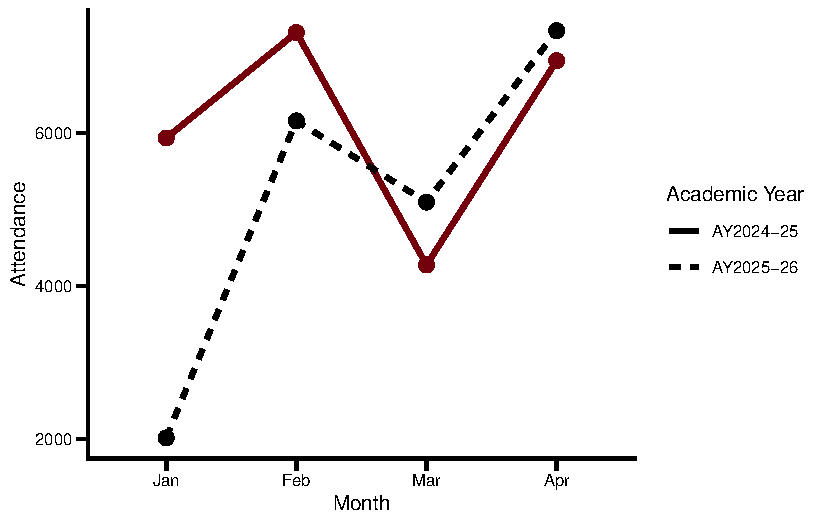
\includegraphics[keepaspectratio]{Monthly-Excutive-Summary-Apr-20260505_files/figure-pdf/MthMthGraph-1.pdf}}

The graph shows that there we fewer students in attendance at Student
Life events as compared to last year. However, during AY2024-25 there
were seveal major events that have not yet happend in AY25-26 (e.g.,
Cockstock was held in January in AY24-25 and will not be held unil March
or later in AY25-26). The point-in-time comparisons that are given each
week account for these events not being held around the same time as
last year.

\raggedright

\textsf{\textbf{\textit{Gender \& Race (Overall)}}}

\begin{table}[!h]
\centering
\caption{\label{tab:ovrllGenRaceTbl}Unique Student Interactions by Race \& Gender}
\centering
\resizebox{\ifdim\width>\linewidth\linewidth\else\width\fi}{!}{
\begin{tabular}[t]{lccc>{}c}
\toprule
\textbf{Race} & \textbf{Female} & \textbf{Male} & \textbf{Unknown} & \textbf{Total}\\
\midrule
White & 3,465 (30.30\%) & 1,722 (15.06\%) & 0 (0.00\%) & \textbf{5,187  (45.36\%)}\\
Race / Ethnicity Unknown & 2,014 (17.61\%) & 637  (5.57\%) & 265 (2.32\%) & \textbf{2,916  (25.50\%)}\\
Black or African American & 979  (8.56\%) & 377  (3.30\%) & 1 (0.01\%) & \textbf{1,357  (11.87\%)}\\
Hispanic & 504  (4.41\%) & 238  (2.08\%) & 0 (0.00\%) & \textbf{742   (6.49\%)}\\
Asian & 335  (2.93\%) & 157  (1.37\%) & 0 (0.00\%) & \textbf{492   (4.30\%)}\\
\addlinespace
Two or More Races & 279  (2.44\%) & 152  (1.33\%) & 0 (0.00\%) & \textbf{431   (3.77\%)}\\
Non-Resident Alien & 160  (1.40\%) & 133  (1.16\%) & 0 (0.00\%) & \textbf{293   (2.56\%)}\\
American Indian or Alaska Native & 9  (0.08\%) & 4  (0.03\%) & 0 (0.00\%) & \textbf{13   (0.11\%)}\\
Native Hawaiian or Other Pacific Islander & 1  (0.01\%) & 2  (0.02\%) & 0 (0.00\%) & \textbf{3   (0.03\%)}\\
\midrule
\textbf{Total} & \textbf{7,746 (67.75\%)} & \textbf{3,422 (29.93\%)} & \textbf{266 (2.33\%)} & \textbf{\textbf{11,434 (100.00\%)}}\\
\bottomrule
\end{tabular}}
\end{table}

\noindent Student Life had total of totalAttend interactions with
uniqueAttend students. Notice also that the majority of our unique
interactions are with female students.

\raggedright

\textsf{\textbf{\textit{Class Standing (Overall)}}}

\noindent Class Standing is determined by the number of course hours
completed, and not by how many years students have completed. The table
shows not only the breakdown by undergraduate class, but also provides
counts for our professional colleges.

\begin{table}[!h]
\centering
\caption{\label{tab:Overall Class Standing Table}Unique Student Interactions by Class Standing}
\centering
\resizebox{\ifdim\width>\linewidth\linewidth\else\width\fi}{!}{
\fontsize{10}{12}\selectfont
\begin{tabular}[t]{lcc}
\toprule
\textbf{Class Standing} & \textbf{Count} & \textbf{Percentage(\%)}\\
\midrule
Sophomore & 2,593 & 22.68\%\\
Unknown & 2,468 & 21.58\%\\
Senior & 2,194 & 19.19\%\\
Junior & 1,893 & 16.56\%\\
Freshman & 1,756 & 15.36\%\\
Graduate & 365 & 3.19\%\\
College of Pharmacy & 77 & 0.67\%\\
Student Affiliate & 66 & 0.58\%\\
Law School & 19 & 0.17\%\\
Medical School & 3 & 0.03\%\\
\midrule
\textbf{Total} & \textbf{11,434} & \textbf{100.00\%}\\
\bottomrule
\end{tabular}}
\end{table}

The most intresting piece of information here is that the Seniors are
more active than the Freshman by less than one percent (\textgreater{}
1\%).

\raggedright

\textsf{\textbf{\textit{Total Interactions by Unit (Overall)}}}

\noindent The table below shows how many total interactions occured by
unit.

\begin{longtable}[t]{lcc}
\caption{Total Interactions by Unit}\tabularnewline

\toprule
\textbf{Unit} & \textbf{Count} & \textbf{Percentage(\%)}\\
\midrule
GE & 14,474 & 70.23\%\\
SG & 2,933 & 14.23\%\\
LSC & 2,181 & 10.58\%\\
CSE & 524 & 2.54\%\\
GMG & 497 & 2.41\%\\
\midrule
\addlinespace
\textbf{Total} & \textbf{20,609} & \textbf{100.00\%}\\
\bottomrule
\end{longtable}




\end{document}
